\documentclass[12pt]{article}
\usepackage{latexblog}

% ============================================================
% Blog Metadata
% ============================================================
\blogtitle{Visual Studio Code for C++ development on MacOS}
\blogdate{2018-12-18}
\blogtags{Visual Studio Code, 开发环境, 闲话编程}
\bloglang{en}
\blogsummary{}

\begin{document}
\makeblogtitle

I've tried lot's of c++ IDEs on MacOS X, but none of them is as powerful as VS Studio on Windows. It's always hard for me to choose an IDE before I want to write some code, as it's called the \emph{Selection phobia}. Generally we have the following choose:

\begin{itemize}
\tightlist
\item
  Vim/Emacs (I'm familiar with VIM but it's still not an easy way, for me)
\item
  CodeBlocks (not good maintained on MacOS)
\item
  CodeLite (it's a good choose!)
\item
  XCode (I just don't like it, \textbf{Heavy} and ugly, can't get used to it)
\item
  QT Creator (it's useful especially when developing Qt projects)
\item
  Eclipse CDT
\item
  NetBeans
\item
  CLion (maybe the best c++ IDE on MaxOS, unfortunately does not have a free version)
\item
  Textmate
\end{itemize}

Recently I tried Visual Studio Code, it's really a good choose for those who want to write some c++ code in a lightweight IDE.

\section{Setup Visual Studio Code for C++ development}\label{setup-visual-studio-code-for-c-development}

First we have to install \href{https://code.visualstudio.com/}{Visual Studio Code}, and a few extensions:

\begin{itemize}
\tightlist
\item
  C/C++
\item
  Easy C++ projects
\end{itemize}

After installed those extensions, reload the editor to activate them. Now we can create a project:

\begin{itemize}
\tightlist
\item
  Choose File \textgreater{} Open folder to open a work directory
\item
  Press F1 and type ``c++'', then select ``Create new C++ project'' command.
\end{itemize}

After the above steps a new project with Makefile is generated.

\section{Common usage}\label{common-usage}

To debug or run the project, just click the button on the bottom status bar, it's easy:

\begin{figure}
\centering
\pandocbounded{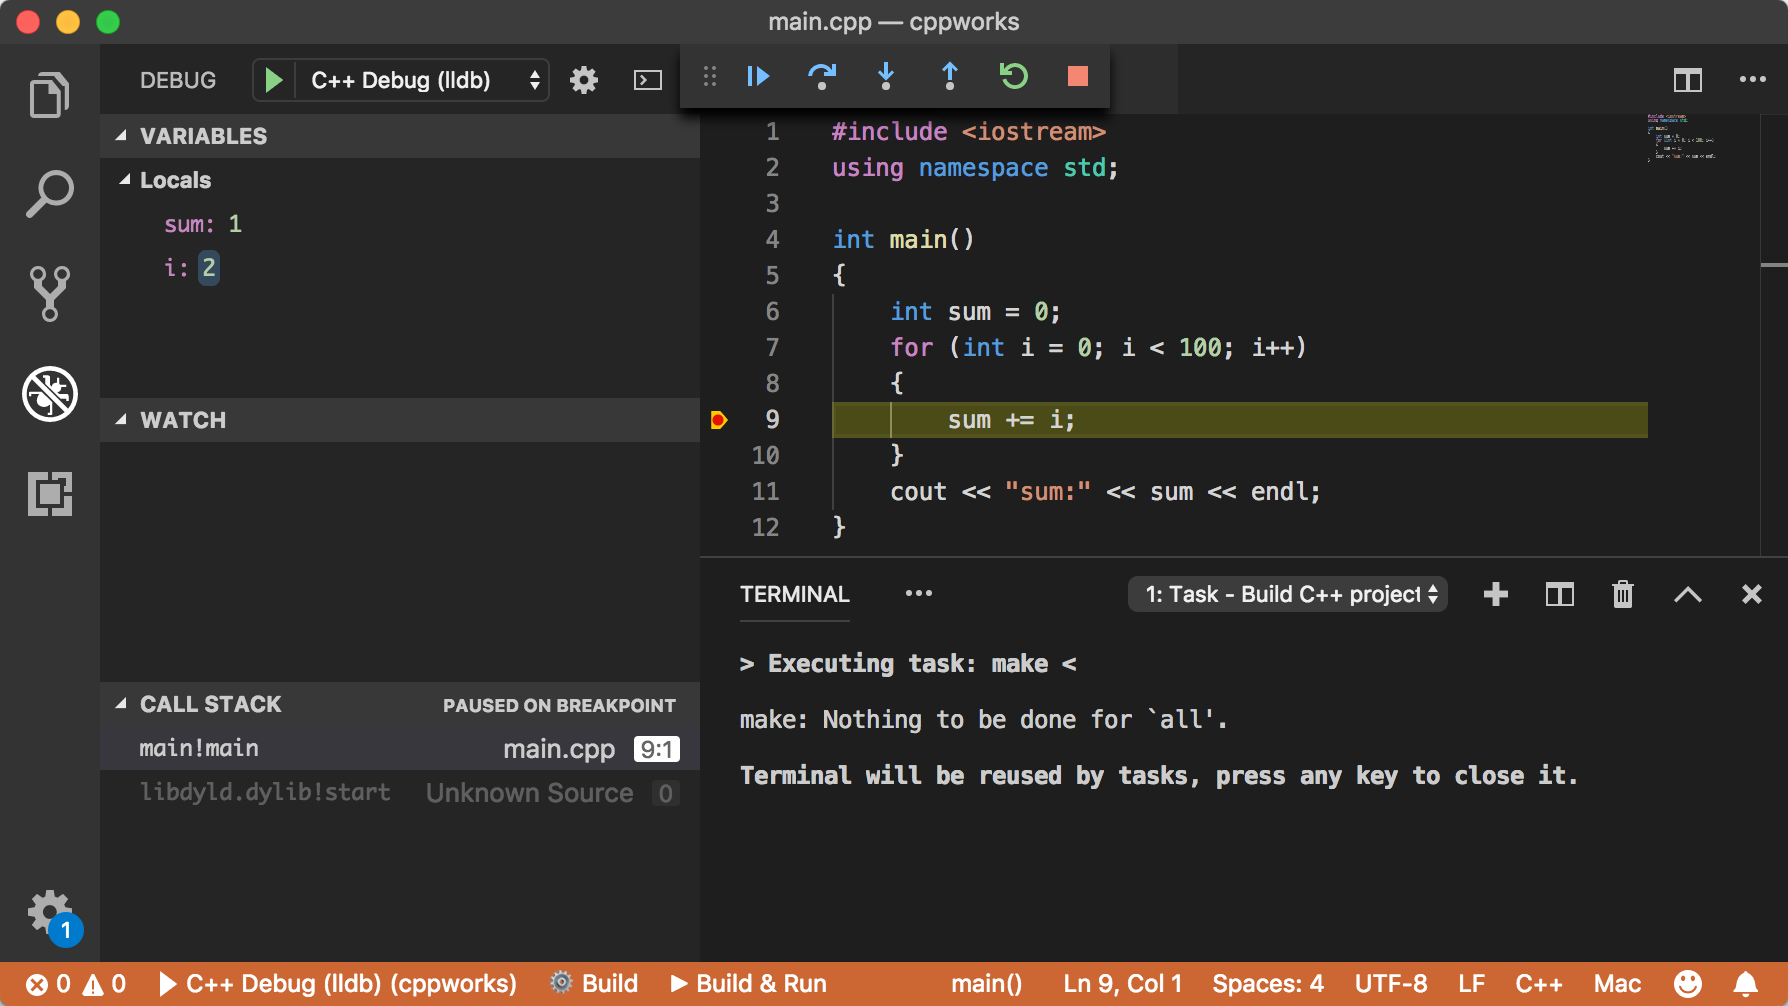
\includegraphics[keepaspectratio,alt={visual code studio snapshot}]{images/vscode_debugging.png}}
\caption{visual code studio snapshot}
\end{figure}

to run other commands, you could just press F1 and guess, for example, to format the code, just search ``format'' and then you got a choice.

\section{Update: How to setup eclipse CDT in MacOX}\label{update-how-to-setup-eclipse-cdt-in-macox}

Recently I tried to use eclipse-cdt with cmake build system, there are a few tips:

\begin{itemize}
\tightlist
\item
  Need to install \texttt{cmake} and \texttt{ninjia}
\item
  Need to start eclipse from command line, this is a \href{https://www.wfbsoftware.de/2019/01/12/eclipse-cdt-c-cmake-on-mac/}{bug}
\end{itemize}

In order to debug, basiclly eclipse only supports gdb, which is has been replaced with lldb in MacOS, so a few setps needed to make it working:

\begin{itemize}
\tightlist
\item
  install gdb via mac ports, \texttt{sudo\ port\ install\ gdb}
\item
  after installed, it's located in \texttt{/opt/local/bin/ggdb}
\item
  create an alias for gdb in your bash profile(eg. \texttt{\textasciitilde{}/.zshrc}), \texttt{alias\ gdb=ggdb}
\item
  codesign for gdb, following \href{https://www.thomasvitale.com/how-to-setup-gdb-and-eclipse-to-debug-c-files-on-macos-sierra/}{How to setup gdb and Eclipse to debug C++ files on macOS Mojave}
\item
  create gdb init file: \texttt{echo\ "set\ startup-with-shell\ off"\ \textgreater{}\ \textasciitilde{}/gdbinit}
\item
  need to start eclipse from terminal, otherwise it will not recongnize gdb
\end{itemize}

Reference:

\begin{itemize}
\tightlist
\item
  \href{https://dev.to/acharluk/developing-c-with-visual-studio-code-4pb9}{Developing C++ with Visual Studio Code}
\end{itemize}


\end{document}
